\section{Reordering}
Another method to decrease memory needed to solve the transport of
photons-electrons reorders the energy groups. When CEPXS generates the cross sections,
it first writes all the cross sections for one particle type and then, the cross
sections for the other particle type into the scattering matrix. Moreover, the
energy range, which is described by the cross sections, is the same for the two
particles. The cross section matrix looks like :
\begin{equation}
S = 
\begin{pmatrix}
A & B\\
C & D
\end{pmatrix}
\end{equation}
where $A$ and $B$ are lower triangular matrices which represents the
scattering for each particle type. The two matrices are lower triangular
because only down scattering is allowed; the cut-off energy forbids the 
thermalization of particles. Matrix B represents the creation of photons by
electrons through bremsstrahlung production and fluorescence production.
Matrix C represents the creation of electrons by photons through photo-electric 
effect, Compton scattering, pair electron production and Auger production 
following photoionization. Now it is important to notice that because 
of energy conservation, a particle can only create a particle which has a 
energy equal or lower than its own. For example, if there are two photons
groups and four electrons groups, the transfers between the groups
look \hbox{like :}
\begin{figure}[H]
\begin{center}
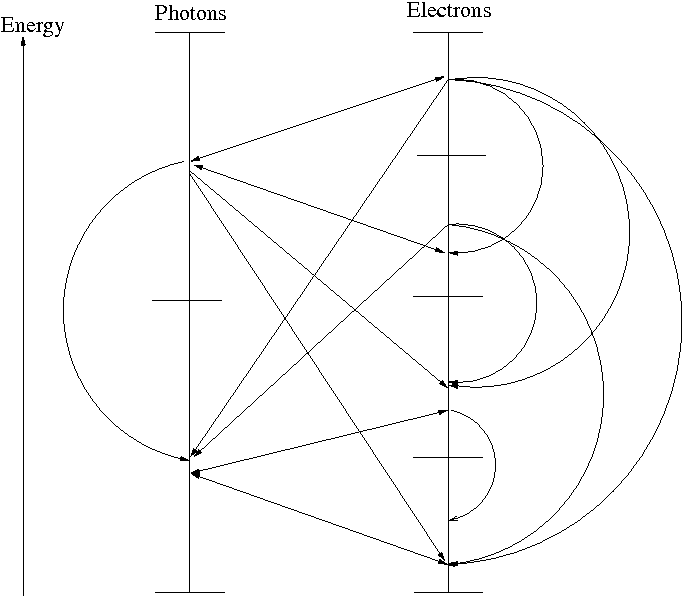
\includegraphics[height=7cm]{group.png}
\caption{Transfer between the different groups}        
\label{joli}
\end{center}
\end{figure}
The pattern of the scattering matrix looks like :
\begin{equation}
S =
\begin{pmatrix}
x & 0 & \vline & x & x & 0 & 0\\
x & x & \vline & x & x & x & x\\
\hline     
x & 0 & \vline & x & 0 & 0 & 0\\
x & 0 & \vline & x & x & 0 & 0\\
x & x & \vline & x & x & x & 0\\
x & x & \vline & x & x & x & x\\
\end{pmatrix}
\end{equation}
We can see that there is no upscattering to the first group of photons, the
first and the second group of electrons coming from the second group of
photons, and the third or the fourth group of electrons (see figure
\ref{joli}). Thus, if we reorder the groups using for the first group \hbox{set :} 
photon group 1, electron group 1, electron group 2 and for the second group 
\hbox{set :} photon group 2, electron group 3, electron group 4. The pattern 
of the scattering matrix looks \hbox{like :}
\begin{equation}
S =
\begin{pmatrix}
x & x & x & \vline & 0 & 0 & 0\\
x & x & 0 & \vline & 0 & 0 & 0\\
x & x & x & \vline & 0 & 0 & 0\\
\hline      
x & x & x & \vline & x & x & x\\
x & x & x & \vline & x & x & 0\\
x & x & x & \vline & x & x & x\\
\end{pmatrix}
\end{equation}
Now, we see that the matrix is block lower triangular and we can solve the
transport problem by solving two problems with only three groups each. 
We can solve the first three groups 
without solving the last three groups since there is no upscattering coming 
from these. Then, we can solve the last three groups, with the first three groups 
hidden in the source term. Thus, we can solve a problem with six groups using the 
same memory that we would use for only three groups. To know how many groups we 
need to gather from each particle in each group set, we can use a simple rule. 
First, we define the number of groups of photons as $n_p$, the number of groups 
electrons as $n_e$ and the greatest common divisor between these two numbers as 
$gcd$. The number of groups of photons to put in a group set is $\frac{n_p}{gcd}$ 
and the number of groups of electrons to put in a group set is $\frac{n_e}{gcd}$. 
Instead of solving one problem of $n$ groups, we can solve $gcd$ problems of 
$\frac{n}{gcd}$ groups.

